\section{Benutzungsschnittstellen}
Es werden Visuelle Darstellungen der Benutzerschnittstellen von der Desktop-Applikation als auch Smartphone-Version gezeigt.
\subsection{Desktop}
Es folgen die Mockups zu der Desktop-Applikationen. Diese dienen als Vorlage für die tatsächliche Realisierung für das Produkt.
\subsubsection{Home Screen}
\begin{figure}[H]
	\centering
	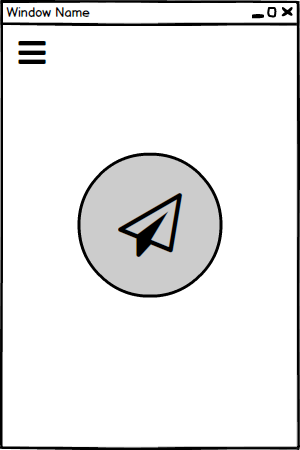
\includegraphics[width=.7\linewidth]{pictures/Desktop/Home.png}\
	\caption{Home Screen der Desktop-Applikation}
\end{figure}
Die Desktop-Applikation soll nicht all zu viel Platz einnehmen weswegen die Größe auf 300 Pixel x 450 Pixel beschränkt wurde. Wie bereits erwähnt gibt es ein simples GUI mit dem man mit nur einem Knopfdruck eine Datei auswählen kann. Ebenfalls hat der Benutzer jederzeit zugriff auf die Optionen welche Links oben mit einem Burger-Menü angezeigt werden.
\subsubsection{Verschlüsselungskey eingeben}
\begin{figure}[H]
	\centering
	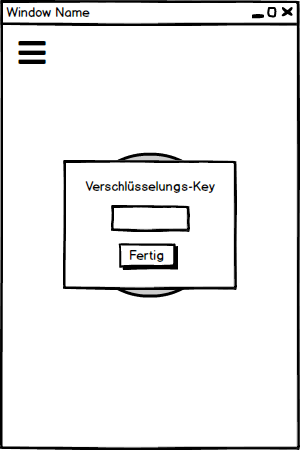
\includegraphics[width=.7\linewidth]{pictures/Desktop/Verschluesselungskey.png}\
	\caption{Eingabefeld des Verschlüsselungskey}
\end{figure}
Bevor dieser Schritt ausgeführt werden kann und der Benutzer zu dieser Schnittstelle kommt muss er, in dem vom Betriebssystem geöffneten File Explorer, die zu versendende Datei auswählen. Wenn dies erfüllt ist kann man einen individuellen Verschlüsselungskey eingegeben werden, welcher dann bei dem Empfänger zur Entschlüsselung der Daten gebraucht wird. Falls sich der Benutzer dazu entscheidet keinen eigenen Schlüssel einzugeben wird der Standardschlüssel, welcher in den Einstellungen zu finden ist, verwendet. In beiden Fällen muss der Benutzer mit einem Knopfdruck auf den "Fertig"-Knopf die Eingabe bestätigen.
\subsubsection{Empfänger auswählen}
\begin{figure}[H]
	\centering
	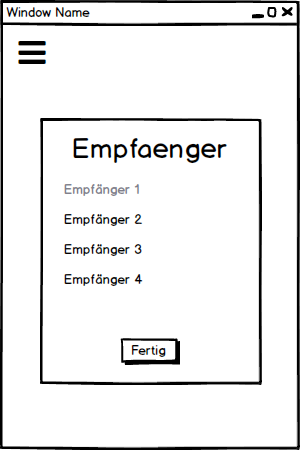
\includegraphics[width=.7\linewidth]{pictures/Desktop/Empfaenger.png}\
	\caption{Empfänger auswählen}
\end{figure}
Nachdem der Schlüssel erfolgreich eingegeben wurde kann der Benutzer nun einen Empfänger auswählen. Hierbei werden ihm alle möglichen Geräte, welche in der Empfangsreichweite sind, angezeigt. Mit einem Knopfdruck auf den Empfängernamen wird er ausgewählt. Dies ist an der Änderung der Farbe erkennbar welche von Schwarz zu Grau wird. Auch hier muss die Auswahl bestätigt werden was mit einem Klick auf den "Fertig"-Knopf getan wird.
\subsubsection{Fortschrittsbalken anzeigen}
\begin{figure}[H]
	\centering
	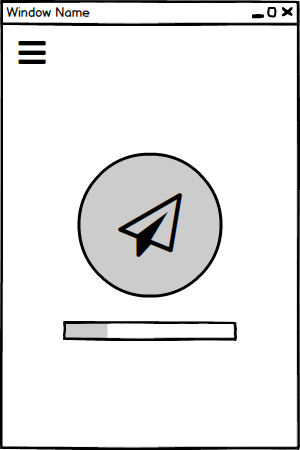
\includegraphics[width=.7\linewidth]{pictures/Desktop/Progress.png}\
	\caption{Fortschrittsbalken anzeigen}
\end{figure}
Wenn nun alle Kriterien für eine erfolgreiche Datenübertragung getroffen wurden, wird die Datei an den zuvor ausgewählten Empfänger gesendet. Dieser Schritt wird auch mit einem Fortschrittsbalken dargestellt.
\subsubsection{Optionen anzeigen}
\begin{figure}[H]
	\centering
	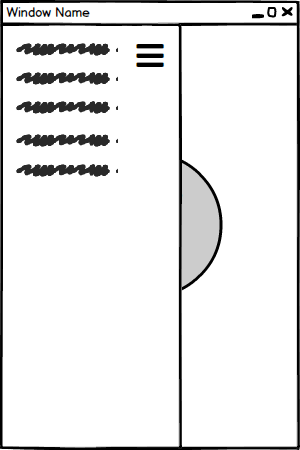
\includegraphics[width=.7\linewidth]{pictures/Desktop/Options.png}\
	\caption{Optionen anzeigen}
\end{figure}
Falls der Benutzer etwas an den Einstellungen ändern möchte, kann dieser zu jedem Zeitpunkt Links oben in der Applikation auf das Burger-Menü klicken was zu einem anzeigen der Optionen führt. Auf der Linken Seite werden dann mehrere Auswahlmöglichkeiten angezeigt. Mit einem Klick auf eine der Optionen komm der Benutzer auf eine neue Seite, wo dann die, zur Einstellung passenden, Informationen angezeigt werden. Um das Menü wieder verschwinden zu lassen kann der Benutzer entweder außerhalb des Optionen Feld klicken oder erneut auf das Burger-Menü drücken. 
\subsubsection{Einstellungen anzeigen}
\begin{figure}[H]
	\centering
	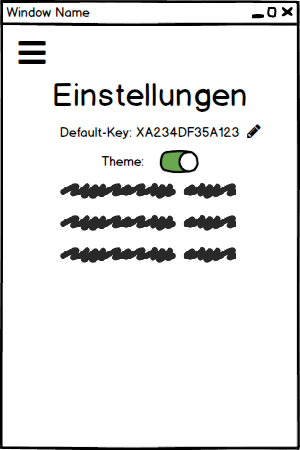
\includegraphics[width=.7\linewidth]{pictures/Desktop/Einstellungen.png}\
	\caption{Einstellungen anzeigen}
\end{figure}
Ein wichtiger Unterpunkt welcher in den Optionen zu sehen ist, sind die Einstellungen. In diesen kann man zum Beispiel den Default-Key sehen oder bei bedarf sogar verändern. Ebenfalls gibt es noch andere Einstellungen welche derzeit mit einem Placeholder belegt sind. Um aus den Einstellungen wieder zum Home Screen zu kommen muss der Benutzer das Burger Menü öffnen auf den Unterpunkt "Home" klicken.
\subsubsection{Nachrichten}
\begin{figure}[H]
	\centering
	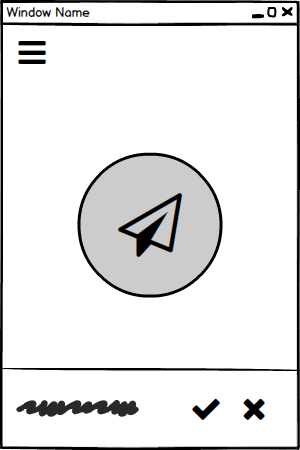
\includegraphics[width=.7\linewidth]{pictures/Desktop/Nachricht.png}\
	\caption{Nachrichten}
\end{figure}
Wenn der Sender nun einen Empfänger ausgewählt hat, erhält dieser eine Nachricht. Diese wird am unteren Rand der Applikation angezeigt und beinhaltet Informationen zum Dateinamen. Neben den Informationen hat der Benutzer 2 Optionen. Das Check Symbol signalisiert das Annehmen der Datei, das Kreuz das Ablehnen. Wenn sich der Benutzer entschieden hat ob er die Datei annehmen oder ablehnen möchte, klickt er einfach auf eines der Symbole. Bei klicken des Kreuzes verschwindet die Nachricht und die Datei kann nicht mehr heruntergeladen werden. Bei anklicken des Check Symbols kommt es zu der nächsten Schnittstelle.
\subsubsection{Nachricht akzeptieren}
\begin{figure}[H]
	\centering
	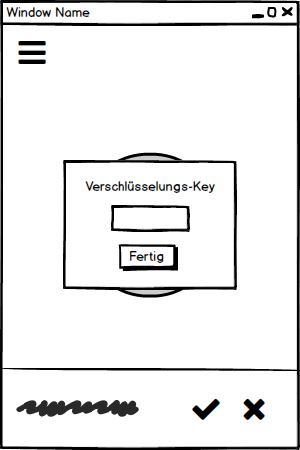
\includegraphics[width=.7\linewidth]{pictures/Desktop/Nachrichtaccept.png}\
	\caption{Nachricht akzeptieren}
\end{figure}
Hat der Empfänger sich dazu entschieden die Datei anzunehmen, kommt wie zuvor schon erwähnt ein Eingabefeld in welchem der gewählte Verschlüsselungskey einzugeben ist. Wenn dieser erfolgreich eingegeben wird und mit einem Klick auf den "Fertig"-Knopf bestätigt wird, wird die übertragene Datei heruntergeladen und kann nun auf dem Gerät des Empfängers geöffnet werden. Gibt es einen Fehler bei der Eingabe des Verschlüsselungskey hat der Benutzer erneut die Chance diesen einzugeben.

\subsection{Smartphone}
Es folgen die Mockups zu der Smartphone-Version der Applikation. Diese dienen als Vorlage für die tatsächliche Realisierung für das Produkt.
\subsubsection{Home Screen}
\begin{figure}[H]
	\centering
	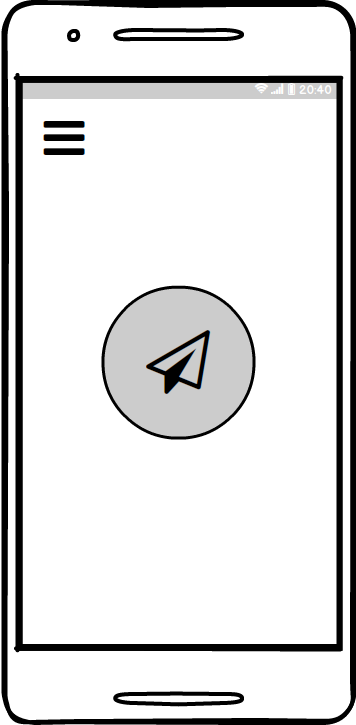
\includegraphics[width=.5\linewidth]{pictures/Mobile/Home.png}\
	\caption{Home Screen der Desktop-Applikation}
\end{figure}
Die Desktop-Applikation soll nicht all zu viel Platz einnehmen weswegen die Größe auf 300 Pixel x 450 Pixel beschränkt wurde. Wie bereits erwähnt gibt es ein simples GUI mit dem man mit nur einem Knopfdruck eine Datei auswählen kann. Ebenfalls hat der Benutzer jederzeit zugriff auf die Optionen welche Links oben mit einem Burger-Menü angezeigt werden.
\subsubsection{Verschlüsselungskey eingeben}
\begin{figure}[H]
	\centering
	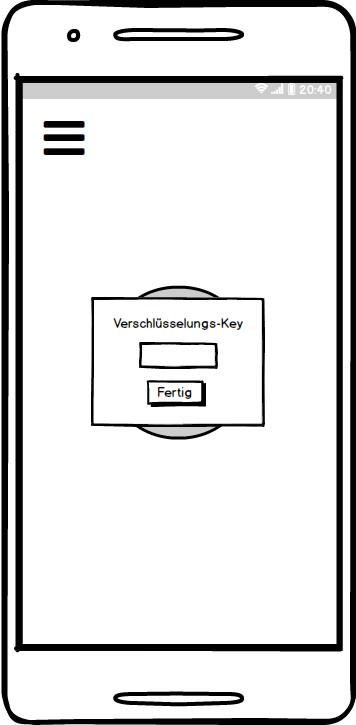
\includegraphics[width=.5\linewidth]{pictures/Mobile/Verschluesselungskey.png}\
	\caption{Eingabefeld des Verschlüsselungskey}
\end{figure}
Bevor dieser Schritt ausgeführt werden kann und der Benutzer zu dieser Schnittstelle kommt muss er, in dem vom Betriebssystem geöffneten File Explorer, die zu versendende Datei auswählen. Wenn dies erfüllt ist kann man einen individuellen Verschlüsselungskey eingegeben werden, welcher dann bei dem Empfänger zur Entschlüsselung der Daten gebraucht wird. Falls sich der Benutzer dazu entscheidet keinen eigenen Schlüssel einzugeben wird der Standardschlüssel, welcher in den Einstellungen zu finden ist, verwendet. In beiden Fällen muss der Benutzer mit einem Knopfdruck auf den "Fertig"-Knopf die Eingabe bestätigen.
\subsubsection{Empfänger auswählen}
\begin{figure}[H]
	\centering
	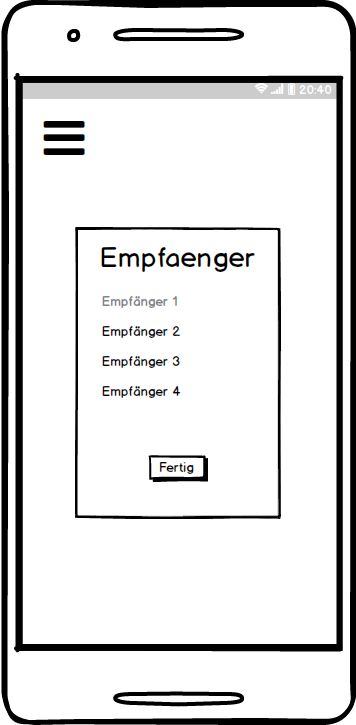
\includegraphics[width=.5\linewidth]{pictures/Mobile/Empfaenger.png}\
	\caption{Empfänger auswählen}
\end{figure}
Nachdem der Schlüssel erfolgreich eingegeben wurde kann der Benutzer nun einen Empfänger auswählen. Hierbei werden ihm alle möglichen Geräte, welche in der Empfangsreichweite sind, angezeigt. Mit einem Knopfdruck auf den Empfängernamen wird er ausgewählt. Dies ist an der Änderung der Farbe erkennbar welche von Schwarz zu Grau wird. Auch hier muss die Auswahl bestätigt werden was mit einem Klick auf den "Fertig"-Knopf getan wird.
\subsubsection{Fortschrittsbalken anzeigen}
\begin{figure}[H]
	\centering
	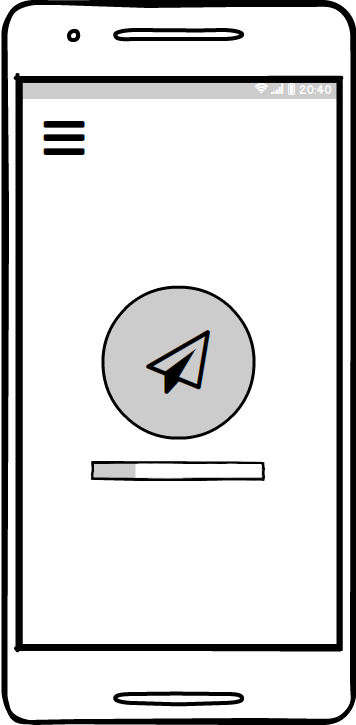
\includegraphics[width=.5\linewidth]{pictures/Mobile/Progress.png}\
	\caption{Fortschrittsbalken anzeigen}
\end{figure}
Wenn nun alle Kriterien für eine erfolgreiche Datenübertragung getroffen wurden, wird die Datei an den zuvor ausgewählten Empfänger gesendet. Dieser Schritt wird auch mit einem Fortschrittsbalken dargestellt.
\subsubsection{Optionen anzeigen}
\begin{figure}[H]
	\centering
	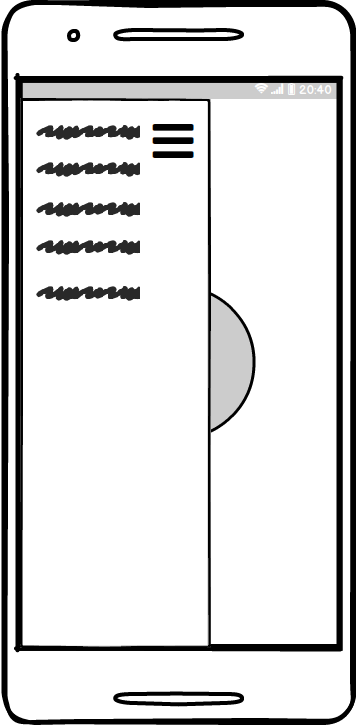
\includegraphics[width=.5\linewidth]{pictures/Mobile/Options.png}\
	\caption{Optionen anzeigen}
\end{figure}
Falls der Benutzer etwas an den Einstellungen ändern möchte, kann dieser zu jedem Zeitpunkt Links oben in der Applikation auf das Burger-Menü klicken was zu einem anzeigen der Optionen führt. Auf der Linken Seite werden dann mehrere Auswahlmöglichkeiten angezeigt. Mit einem Klick auf eine der Optionen komm der Benutzer auf eine neue Seite, wo dann die, zur Einstellung passenden, Informationen angezeigt werden. Um das Menü wieder verschwinden zu lassen kann der Benutzer entweder außerhalb des Optionen Feld klicken oder erneut auf das Burger-Menü drücken. 
\subsubsection{Einstellungen anzeigen}
\begin{figure}[H]
	\centering
	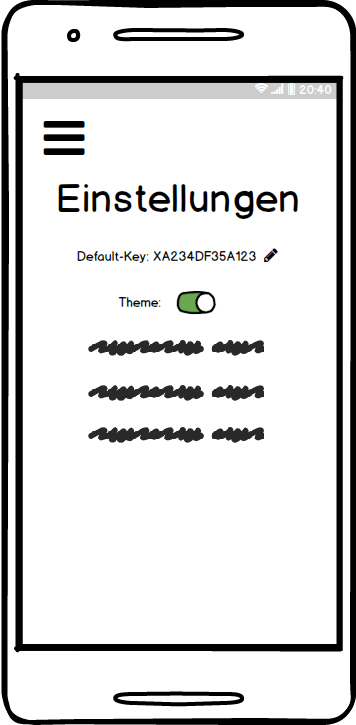
\includegraphics[width=.5\linewidth]{pictures/Mobile/Einstellungen.png}\
	\caption{Einstellungen anzeigen}
\end{figure}
Ein wichtiger Unterpunkt welcher in den Optionen zu sehen ist, sind die Einstellungen. In diesen kann man zum Beispiel den Default-Key sehen oder bei bedarf sogar verändern. Ebenfalls gibt es noch andere Einstellungen welche derzeit mit einem Placeholder belegt sind. Um aus den Einstellungen wieder zum Home Screen zu kommen muss der Benutzer das Burger Menü öffnen auf den Unterpunkt "Home" klicken.
\subsubsection{Nachrichten}
\begin{figure}[H]
	\centering
	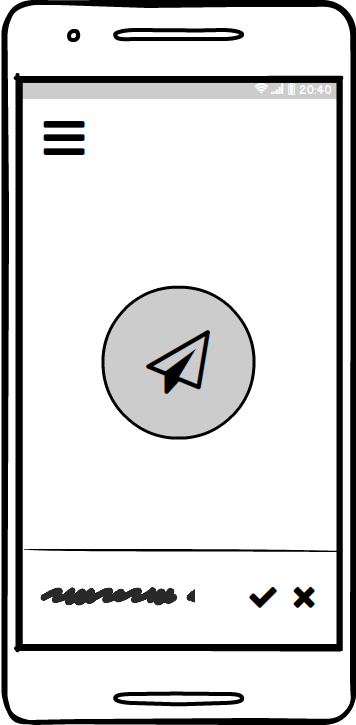
\includegraphics[width=.5\linewidth]{pictures/Mobile/Nachricht.png}\
	\caption{Nachrichten}
\end{figure}
Wenn der Sender nun einen Empfänger ausgewählt hat, erhält dieser eine Nachricht. Diese wird am unteren Rand der Applikation angezeigt und beinhaltet Informationen zum Dateinamen. Neben den Informationen hat der Benutzer 2 Optionen. Das Check Symbol signalisiert das Annehmen der Datei, das Kreuz das Ablehnen. Wenn sich der Benutzer entschieden hat ob er die Datei annehmen oder ablehnen möchte, klickt er einfach auf eines der Symbole. Bei klicken des Kreuzes verschwindet die Nachricht und die Datei kann nicht mehr heruntergeladen werden. Bei anklicken des Check Symbols kommt es zu der nächsten Schnittstelle.
\subsubsection{Nachricht akzeptieren}
\begin{figure}[H]
	\centering
	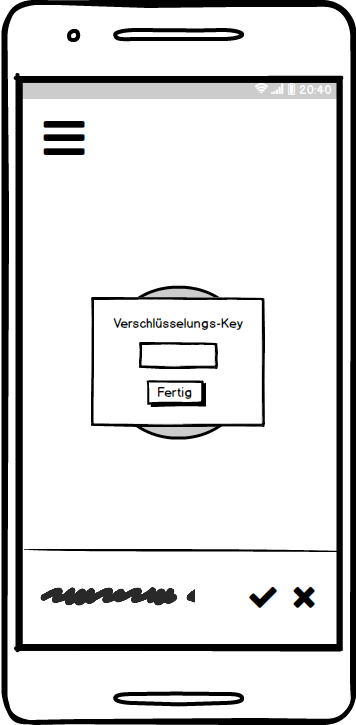
\includegraphics[width=.5\linewidth]{pictures/Mobile/Nachrichtaccept.png}\
	\caption{Nachricht akzeptieren}
\end{figure}
Hat der Empfänger sich dazu entschieden die Datei anzunehmen, kommt wie zuvor schon erwähnt ein Eingabefeld in welchem der gewählte Verschlüsselungskey einzugeben ist. Wenn dieser erfolgreich eingegeben wird und mit einem Klick auf den "Fertig"-Knopf bestätigt wird, wird die übertragene Datei heruntergeladen und kann nun auf dem Gerät des Empfängers geöffnet werden. Gibt es einen Fehler bei der Eingabe des Verschlüsselungskey hat der Benutzer erneut die Chance diesen einzugeben.